\chapter{Stratégies de redressement : recherche, comparaison, robustesse}
\label{ch:strategie}

\section{Point de départ : des objectifs qui ne sont pas tous compatibles}

La mission fixe douze objectifs simultanés : moins de chômage, plus de niveau de vie médian, moins de pauvreté, plus de
pouvoir d'achat, de productivité, de croissance et de compétitivité, moins de déficit et de dette, une meilleure balance
commerciale, plus de souveraineté industrielle et énergétique, une protection sociale soutenable. Les expériences des
chapitres précédents montrent que ces objectifs entrent en tension :

\begin{itemize}
\item \textbf{déficit contre activité à court terme} : toute consolidation budgétaire réduit l'activité la première année
(de 0,3 à 2,1~\% de PIB par point de solde gagné selon l'instrument) ;
\item \textbf{déficit contre pouvoir d'achat} : les instruments les moins coûteux en activité (TVA, taxe carbone,
désindexation) réduisent le pouvoir d'achat de tous les ménages et pèsent davantage sur les modestes ;
\item \textbf{pauvreté contre déficit} : les prestations ciblées réduisent efficacement la pauvreté mais coûtent ;
\item \textbf{production à long terme contre chômage à court terme} : allonger la durée du travail ou les carrières
augmente la production à long terme mais d'abord le chômage ;
\item \textbf{souveraineté industrielle contre pouvoir d'achat} : relocaliser renchérit les produits ; protéger par des
droits de douane fait payer les consommateurs et les exportateurs ;
\item \textbf{dette contre investissement} : l'investissement public est le seul levier de dépense qui accroît durablement
la production, mais il ne s'autofinance pas.
\end{itemize}

Le modèle ne peut pas arbitrer entre ces objectifs : c'est un choix de société. Il peut en revanche chercher, pour une
pondération explicite des objectifs, les combinaisons de mesures qui donnent le meilleur résultat, et vérifier leur
cohérence. C'est ce que fait ce chapitre.

\section{Méthode : un méta-modèle linéaire et une optimisation sous contraintes}

\paragraph{Étape 1 : méta-modèle.} Chaque levier est représenté par la pente de ses effets, mesurée sur les expériences
des chapitres~\ref{ch:experiences} et~\ref{ch:complementaires} : effet par unité de curseur sur chaque indicateur (PIB,
emploi, chômage, solde, dette, solde extérieur, revenu national, industrie, pouvoir d'achat, pauvreté, médiane, inflation)
et chaque horizon (2029, 2030, 2032, 2037, 2047). Les hausses et les baisses d'un même levier ont des pentes distinctes.
L'effet d'un programme est approché par la somme des effets de ses mesures.

\paragraph{Étape 2 : programmes linéaires.} Pour chaque scénario, on maximise une fonction objectif linéaire sous
contraintes linéaires (méthode HiGHS, bibliothèque scipy), pour chacune des quatre règles d'âge de départ (64 ans,
actuelle ; 62, 65 et 66 ans) ; la meilleure est retenue. Une \textbf{pénalité de parcimonie} (coût fixe par levier
utilisé à pleine amplitude) évite les programmes qui actionnent tous les leviers d'un epsilon.

\paragraph{Contraintes de faisabilité communes} (hypothèses explicites, identiques pour tous les scénarios) :
\begin{itemize}
\item amplitude de chaque levier limitée à la plage testée par les expériences (pas d'extrapolation au-delà) ;
\item hausses de prélèvements limitées à 1,5 point de PIB et économies de dépenses à 2,5 points de PIB (effet sur le
solde en 2030), sur un mandat ;
\item \textbf{leviers exclus} : hausse de l'IS et des impôts de production (leur coût passe par la délocalisation des
bénéfices et des activités, que le modèle ne représente pas : il en sous-estimerait le coût) ; réindustrialisation
(c'est un objectif, pas un instrument : le modèle n'en représente pas le coût public) ; SMIC (l'emploi peu qualifié n'est
pas représenté).
\end{itemize}

\paragraph{Étape 3 : vérification.} Chaque programme est re-simulé avec le modèle complet (microsimulation comprise),
puis soumis à sept chocs d'environnement et à une mise en œuvre partielle.

\begin{table}[htbp]
\centering\small
\caption{Fonctions objectifs et contraintes des scénarios (écarts à la référence).}
\label{tab:objectifs}
\begin{tabularx}{\linewidth}{@{}p{2.4cm}LL@{}}
\toprule
Scénario & Objectif maximisé & Contraintes \\
\midrule
A — budgétaire & Réduire la dette en 2037 & PIB 2030 $\geq -0{,}5$~\% ; chômage 2030 $\leq$ +0,3 pt ; pauvreté 2037 $\leq 0$ ; pouvoir d'achat 2030 $\geq -1$~\% \\
B — croissance & PIB 2037 + part de l'industrie 2037 & dette 2037 $\leq 0$ ; solde 2030 $\geq 0$ ; pauvreté $\leq$ +0,2 pt \\
C — équilibré & PIB 2037 + emploi 2037 / 200\,000 $-$ 2 $\times$ pauvreté + pouvoir d'achat 2037 & dette 2037 $\leq -5$ pt ; solde 2030 $\geq$ +0,5 pt ; pauvreté $\leq 0$ ; chômage 2030 $\leq$ +0,2 pt \\
D — effort maximal & Réduire la dette en 2047 & plafonds relevés à 2,5 pt (impôts) et 4 pt (dépenses) ; PIB 2030 $\geq -1{,}5$~\% ; pauvreté $\leq 0$ \\
\bottomrule
\end{tabularx}
\end{table}

\begin{encadre}{Encadré 7.1 — Ce qu'une optimisation peut et ne peut pas dire}
Un programme « optimal » au sens mathématique est la meilleure combinaison \emph{pour la fonction objectif choisie, dans
le modèle, avec ses hypothèses}. Changer la pondération des objectifs change la solution ; changer une hypothèse du modèle
(fermeture d'offre, élasticités) aussi. L'optimiseur a en outre tendance à exploiter les angles morts du modèle : lors des
premiers essais, il choisissait massivement les hausses d'IS et d'impôts de production, dont le modèle ne voit pas le
coût, ou retenait le retour à 62 ans pour réduire le chômage (moins d'actifs), ce qui n'a pas de sens économique. Ces
solutions ont été écartées par les exclusions et contraintes décrites plus haut. \textbf{Aucune des solutions ci-dessous
n'est un optimum politique ou social.}
\end{encadre}

\section{Les quatre programmes}

\begin{table}[htbp]
\centering\small
\caption{Leviers retenus par l'optimisation (valeur du curseur ; « -- » : inchangé). La colonne R, programme recommandé, est présentée au
chapitre~\ref{ch:synthese}.}
\label{tab:scmesures}
\tabfit{../tableaux/scenarios_mesures}
\end{table}

\paragraph{Scénario A — redressement budgétaire prioritaire.} L'optimiseur combine des hausses d'impôts sur la
consommation (TVA +2 points au taux normal et aux taux réduits, taxe carbone +23~€/t), les droits de succession (+50~\%),
une hausse des cotisations employeurs (+10\md) et une baisse de l'investissement public ($-$10\md), et utilise une partie
de la marge pour la prime d'activité (+25~\%) — qui neutralise l'effet des taxes sur la pauvreté — et un peu de
dépense de fonctionnement (+2,4\md) qui limite la perte d'activité. Âge de départ inchangé.

\paragraph{Scénario B — croissance et réindustrialisation prioritaires.} Le report de l'âge à 66 ans, l'investissement
public (+30\md) et le passage aux 37 heures sont les moteurs de la croissance ; ils sont financés par la TVA, les droits
de succession, les cotisations, la baisse des allocations chômage ($-$25~\%). La réindustrialisation n'étant pas un
instrument, l'objectif « industrie » est peu sensible aux leviers disponibles.

\paragraph{Scénario C — redressement équilibré.} Il combine une forte redistribution vers les ménages modestes (RSA,
prime d'activité, allocations familiales et minimum vieillesse +25~\%, baisse de la TVA de 0,9 point et de la CSG d'un
point), financée par les impôts sur le patrimoine et le capital (ISF à 1~\%, PFU +15 points, successions +50~\%), les
cotisations employeurs et la baisse des allocations chômage ; le report de l'âge à 66 ans soutient la production à long
terme. 50\,000 emplois publics sont créés, l'investissement public baisse de 10\md.

\paragraph{Scénario D — effort maximal sur la dette.} Avec des plafonds relevés, l'optimiseur mobilise presque tous les
leviers de recettes et d'économies : TVA, CSG, IR, ISF, PFU, successions, taxe carbone (+54~€/t), cotisations, fonctionnement
($-$13,6\md), investissement public, sous-indexation des pensions, allocations chômage, durée du travail (37 heures),
droits de douane ; il préserve la pauvreté par la prime d'activité et les allocations familiales.

\section{Vérification avec le modèle complet}

Le méta-modèle additif reproduit le modèle complet à quelques centièmes près pour A et C, et à quelques dixièmes près pour
B et D, qui combinent des chocs d'offre et de prix :
\begin{center}\small
\begin{tabular}{@{}lrrrrrrrr@{}}
\toprule
 & \multicolumn{2}{c}{PIB 2030 (\%)} & \multicolumn{2}{c}{PIB 2037 (\%)} & \multicolumn{2}{c}{Dette 2037 (pt)} & \multicolumn{2}{c}{Dette 2047 (pt)} \\
 & méta & complet & méta & complet & méta & complet & méta & complet \\
\midrule
A & $-$0,43 & $-$0,43 & $-$0,19 & $-$0,19 & $-$14,9 & $-$14,9 & $-$44,7 & $-$43,5 \\
B & +0,93 & +0,88 & +1,79 & +1,77 & 0,0 & $-$0,3 & $-$0,8 & $-$2,7 \\
C & +0,36 & +0,36 & +1,00 & +1,00 & $-$5,7 & $-$5,7 & $-$14,0 & $-$14,3 \\
D & $-$1,50 & $-$1,46 & $-$0,24 & $-$0,23 & $-$28,0 & $-$28,1 & $-$95,9 & $-$89,9 \\
\bottomrule
\end{tabular}
\end{center}

\section{Résultats aux quatre horizons}

\begin{figure}[htbp]
\centering
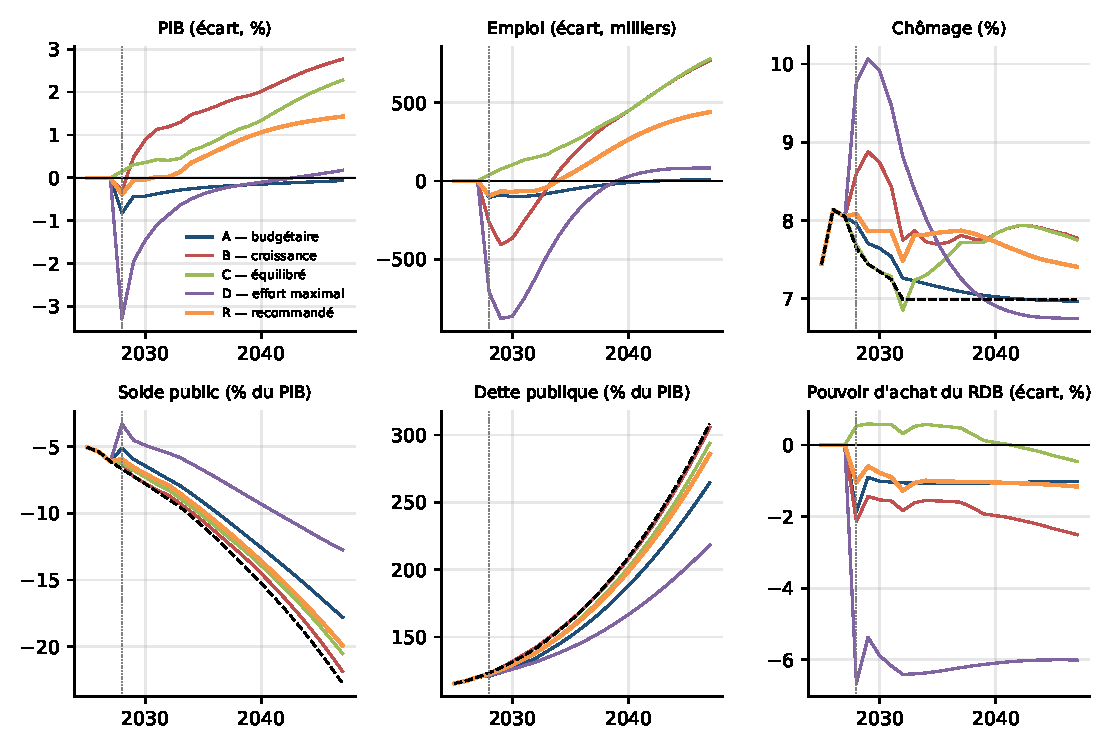
\includegraphics[width=\linewidth]{scenarios.pdf}
\caption{Trajectoires des scénarios (modèle complet). Les panneaux du chômage, du solde et de la dette donnent les niveaux,
avec la référence en tirets ; les autres, les écarts à la référence. Les mesures commencent en 2028.}
\label{fig:scenarios}
\end{figure}

\begin{table}[p]
\centering\scriptsize
\caption{Scénario A — redressement budgétaire prioritaire (modèle complet).}\label{tab:scA}
\tabfit{../tableaux/scenario_A}\\[10pt]
\caption{Scénario B — croissance et réindustrialisation prioritaires.}\label{tab:scB}
\tabfit{../tableaux/scenario_B}
\end{table}

\begin{table}[p]
\centering\scriptsize
\caption{Scénario C — redressement équilibré.}\label{tab:scC}
\tabfit{../tableaux/scenario_C}\\[10pt]
\caption{Scénario D — effort maximal sur la dette.}\label{tab:scD}
\tabfit{../tableaux/scenario_D}
\end{table}

\paragraph{Scénario A.} \emph{Court terme (2029-2030)} : le solde s'améliore de 1,3 point de PIB, au prix d'un PIB plus
bas de 0,43~\%, de 88\,000 à 101\,000 emplois en moins (chômage +0,3 point) et d'un pouvoir d'achat réduit d'un point ;
les prix sont plus élevés de 2,4~\% (TVA, taxe carbone). \emph{Moyen et long terme} : la perte d'activité s'estompe
($-$0,19~\% en 2037), l'amélioration du solde s'accumule (+2,1 points en 2037, +5 en 2047 grâce aux intérêts
économisés), la dette est plus basse de 15 points en 2037 et de 44 points en 2047. \emph{Distribution} : la pauvreté
baisse légèrement ($-$0,24 point) grâce à la prime d'activité, mais le premier décile perd 3,2~\% de niveau de vie (ménages
sans revenu d'activité, qui subissent la TVA sans bénéficier de la prime d'activité) et les déciles 6 à 10 perdent 1 à
2,3~\%. \textbf{Le coût porte sur le pouvoir d'achat, de façon durable} ($-$1~\% jusqu'en 2047).

\paragraph{Scénario B.} \emph{Court terme} : le PIB augmente (+0,5 à +0,9~\%) grâce à l'investissement public, mais
\textbf{le passage aux 37 heures détruit d'abord 409\,000 emplois} (chômage 8,9~\% en 2029 au lieu de 7,4~\%) : la
production par salarié augmente plus vite que la demande. \emph{Moyen terme} : le chômage reflue (7,8~\% en 2032) et le PIB
progresse (+1,2~\% en 2032, +1,8~\% en 2037, +2,8~\% en 2047) ; l'emploi devient supérieur à la référence à partir de
2035 environ (+293\,000 en 2037). \emph{Finances publiques} : neutres par construction (contrainte dette 2037 $\leq 0$).
\emph{Pouvoir d'achat} : $-$1,4 à $-$2,5~\%, car le salaire horaire baisse (37 heures payées 35) et les prix diminuent moins
que les revenus des ménages. Le chômage reste plus élevé que dans la référence de 0,8 point jusqu'en 2047, parce que la
population active augmente continûment avec le report progressif à 66 ans : l'économie absorbe les actifs supplémentaires
avec retard. Pauvreté +0,38 point (statique). \textbf{Le scénario B achète de la production future avec du chômage et
du pouvoir d'achat présents.}

\paragraph{Scénario C.} \emph{Court terme} : PIB +0,3~\%, emploi +75\,000 à +104\,000, chômage stable, pouvoir d'achat
+0,6~\%, solde +0,5 point. \emph{Long terme} : PIB +1,0~\% en 2037 et +2,3~\% en 2047 (report de l'âge), dette $-$5,7 points
en 2037 et $-$14 points en 2047. \emph{Distribution} : c'est le scénario le plus redistributif : pauvreté $-$2,9 points,
indice de Gini $-$1,7 point, niveau de vie médian +4,2~\% (statique) ; le premier décile gagne 11,7~\%, le dernier perd
1,1~\%. \emph{Points faibles} : la consolidation est modeste (+0,5 à +0,9 point de solde) ; à partir de 2035, le chômage
dépasse celui de la référence (+0,7 point) pour la même raison que dans B (report de l'âge) ; la baisse des allocations
chômage repose sur une hypothèse non estimée.

\paragraph{Scénario D.} \emph{Court terme} : récession marquée, PIB $-$2,0~\% en 2029, 879\,000 emplois en moins
(chômage 10,1~\%), pouvoir d'achat $-$5,4~\%. \emph{Long terme} : le PIB revient à la référence vers 2040 ; le solde
s'améliore de 2,7 points dès 2029 et de 4,9 points en 2037 ; la dette est plus basse de 28 points en 2037 (151~\% au lieu
de 179~\%) et de 90 points en 2047. Le pouvoir d'achat reste inférieur de 6~\% à la référence. Tous les déciles perdent
(de 1,3 à 6,8~\%). \textbf{Le scénario D montre ce que coûte, dans le modèle, une stabilisation rapide de la dette :
une récession de deux ans et une baisse durable du pouvoir d'achat.}

\begin{figure}[htbp]
\centering
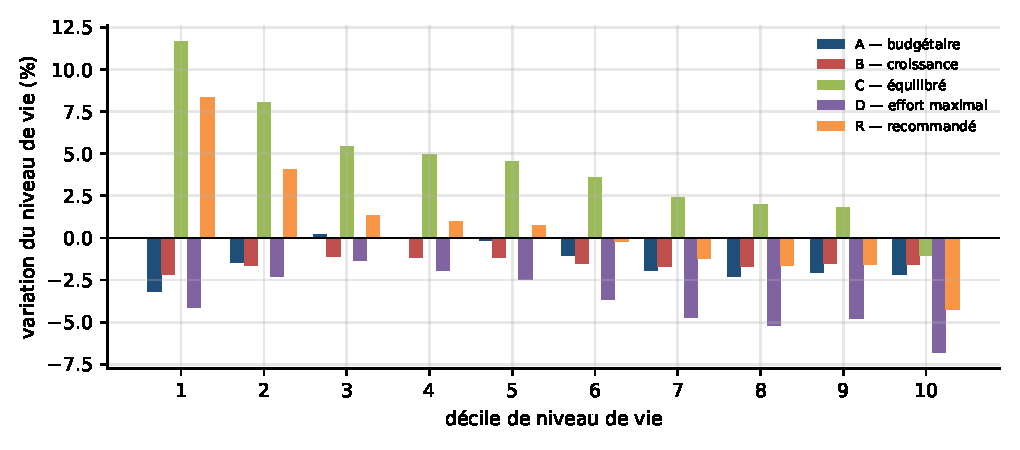
\includegraphics[width=0.95\linewidth]{scenarios_distribution.pdf}
\caption{Variation statique du niveau de vie par décile dans chaque scénario (microsimulation ; mesures fiscales et
sociales seulement, hors effets macroéconomiques).}
\label{fig:scdist}
\end{figure}

\begin{resultat}[Le constat central : aucun scénario ne stabilise la dette]
Dans les cinq scénarios, la dette publique continue d'augmenter en part du PIB jusqu'en 2047 (de 151~\% à 179~\% du PIB en
2037, de 218~\% à 306~\% en 2047). La référence suppose un taux d'intérêt de 4,89~\% maintenu vingt ans et une croissance
nominale d'environ 3~\% : avec une dette de 130~\% du PIB, stabiliser le ratio exige un excédent primaire d'environ
2,5 points de PIB, alors que la référence affiche un déficit primaire de 3,4 points en 2030. L'effort nécessaire, de
l'ordre de 6 points de PIB, dépasse ce que les leviers testés peuvent apporter sans récession majeure (scénario D :
2,9 points en 2030, avec un PIB plus bas de 1,5~\%). Deux conclusions s'imposent : (1) la soutenabilité de la dette
dépend d'abord du taux d'intérêt et de la croissance, plus que de toute réforme isolée ; (2) les niveaux de dette de très
long terme du modèle ne doivent pas être lus comme des prévisions. \fiab{robuste} pour le sens ; \fiab{fragile} pour les
niveaux.
\end{resultat}

\section{Robustesse}

\paragraph{Sept chocs d'environnement.} Chaque scénario et la référence ont été simulés sous sept hypothèses défavorables
appliquées à partir de 2028 : croissance mondiale plus faible (demande adressée $-$1~\% par an, cumulé) ; crise énergétique
(énergie importée +50~\% dès 2029) ; hausse des taux longs de 1,5 point ; inflation importée persistante (+2~\% par an de
2028 à 2032) ; dégradation de la compétitivité (prix des concurrents $-$5~\%) ; productivité plus faible ($-$0,3 point par
an) ; choc démographique (population active $-$0,2~\% par an).

\begin{table}[htbp]
\centering\scriptsize
\caption{Robustesse : écarts à la référence (soumise au même choc) en 2037. PIB en \%, dette en points de PIB.}
\label{tab:robustesse}
\tabfit{../tableaux/scenarios_robustesse}
\end{table}

\begin{table}[htbp]
\centering\scriptsize
\caption{Niveau de la dette publique en 2037 (\% du PIB) selon les chocs.}
\label{tab:dettechocs}
\tabfit{../tableaux/scenarios_dette_niveaux}
\end{table}

\paragraph{Lecture.} (1) \textbf{Les écarts aux références sont remarquablement stables} d'un choc à l'autre : les effets
des programmes s'ajoutent à ceux des chocs, sans interaction forte, parce que le modèle est proche de la linéarité pour
des chocs de cette taille. La hausse des taux \emph{renforce} les gains de dette des programmes de consolidation (A : $-$15,5
points au lieu de $-$14,9 ; D : $-$29,1 au lieu de $-$28,1) : chaque point de déficit évité économise davantage d'intérêts.
(2) \textbf{Les niveaux, en revanche, varient fortement} (tableau~\ref{tab:dettechocs}) : une crise énergétique ou une
hausse des taux ajoute environ 12 points de dette en 2037 dans tous les scénarios, autant que le gain du scénario A. Un
programme de redressement doit donc disposer de marges face aux chocs. (3) Les tests « productivité » et « démographie »
donnent des résultats paradoxaux pour la référence (moins de dette quand la productivité ou la population active
baissent) qui révèlent une limite du modèle (section~\ref{sec:paradoxe}) : ils ne sont pas interprétés.
(4) Ces tests ne couvrent pas l'incertitude sur les paramètres du modèle lui-même (fermeture d'offre, élasticités),
traitée par la contre-expertise : les effets sur le PIB et l'emploi au-delà de cinq ans des scénarios qui reportent l'âge
(B, C) sont \fiab{fragiles}.

\paragraph{Difficultés de mise en œuvre.} Si chaque mesure n'est mise en œuvre qu'à moitié, les effets sont presque
exactement divisés par deux (dernière ligne du tableau~\ref{tab:robustesse}) : A donne $-$7,7 points de dette en 2037 au lieu
de $-$14,9 ; C, $-$3,0 au lieu de $-$5,7. Les programmes ne présentent pas d'effet de seuil : une mise en œuvre partielle
réduit les gains sans les annuler. Les délais de mise en œuvre sont représentés de façon simplifiée : application au
1\textsuperscript{er} janvier 2028, montée en charge sur cinq ans pour les emplois publics et la réindustrialisation, deux
ans pour la durée du travail, une génération pour l'âge de départ.

\section{Contradictions et arbitrages mis en évidence}

\begin{enumerate}
\item \textbf{Il n'existe pas, dans le modèle, de programme qui améliore à la fois le solde, l'activité, le pouvoir
d'achat et la pauvreté à court terme.} A améliore le solde au prix du pouvoir d'achat ; B l'activité future au prix du
chômage présent ; C la pauvreté et l'activité au prix d'une consolidation faible ; D la dette au prix d'une récession.
\item \textbf{La pauvreté peut être réduite à faible coût} par des prestations ciblées sur les ménages modestes en emploi
(prime d'activité) ou sans emploi (RSA, minimum vieillesse), même dans un programme de consolidation : c'est l'arbitrage
le moins coûteux du modèle.
\item \textbf{Le report de l'âge de départ est le levier de croissance le plus puissant à long terme}, mais ses effets sur
l'emploi et la dette dépendent de l'hypothèse de bouclage et il augmente d'abord le chômage.
\item \textbf{La souveraineté industrielle n'est pas atteignable avec les instruments du modèle} : la réindustrialisation
y est un objectif exogène, et la protection commerciale la contrarie.
\item \textbf{La soutenabilité de la dette dépend surtout des taux et de la croissance} ; aucun programme réaliste ne la
garantit seul si le taux reste proche de 5~\%.
\end{enumerate}
